\documentclass[letterpaper,12pt]{article}
\usepackage[margin=1in]{geometry}
\usepackage{graphicx}  % Include figure files
\usepackage{xcolor}  % Allow for a color text
\usepackage{amsmath}  % math fonts
\usepackage{amsfonts}  % math fonts
\usepackage{latexsym}  % math fonts
\usepackage{amssymb}  % math fonts
\usepackage{mathtools} % Give more control of how equations are displayed
\usepackage{appendix} % Lets you create an appendix
\usepackage[numbered]{matlab-prettifier} % Let's me import MATLAB code in a nice format
\usepackage{indentfirst} % This indents the first paragraph. By default latex won't do it.

\setlength{\parskip}{1em} % This skips a line when making new paragraphs
\newtagform{show_eq}{(Eq.\ }{)}  % how the equation numbers are displayed
\usetagform{show_eq} % this goes with the \newtagform

\begin{document}

% ================================== Title Page ==========================================
\begin{titlepage}
 \begin{center}
 \vspace*{1in}
{\Huge Comparison Between Experimental and Analytical Operational Amplifier in a Closed Loop Configuration Models}\\
    \bigskip
    by\\
    \bigskip
    {\Large Kevin Moran} \\
    \bigskip
    Lab Partner : Jorge\\
    Date of Experiment : Thursday, October 14th, 2020

    \bigskip\bigskip\bigskip
    University of Southern California\\
    Aerospace and Mechanical Engineering Department\\
    AME 341A : Mechoptronics
 \end{center}
\end{titlepage}


% ================================== Main Text =====================================


% --------------------------------- Introduction -----------------------------------
\section{Introduction}
Operational Amplifiers, often referred to as \textit{op-amps}, are a vital part of data acquisition circuits and circuits that rely on threshold voltage inputs to activate additional components. As the name suggest, om-amps serve as voltage amplifiers and can be setup in various configurations using passive circuit elements such as resistors and capacitors. Figure \ref{NFL} illustrates a LM741 op-amp in a negative feedback loop configuration.

\begin{figure}[ht]
    \centering
    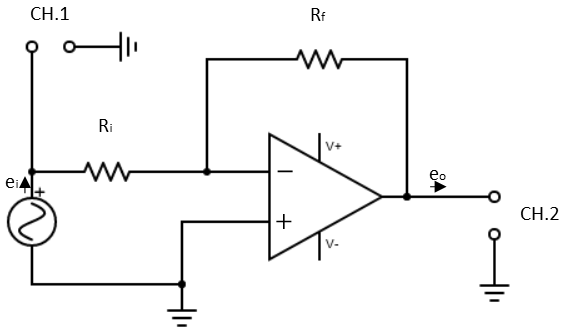
\includegraphics[scale=1.25]{feedback.png}
    \caption{\small LM741 operation amplifier negative feedback loop schematic. All components of the circuit are grounded using a common ground. CH1 and CH2 represent probe connection on Vbench Interface.}
    \label{NFL}
\end{figure}
% ~~~~~~~~~~~~~~~~~~~~~~~~~~~~~~~ Gain ~~~~~~~~~~~~~~~~~~~~~~~~~~~~~~~~~~~~~~~~~~~~
\subsection{Gain}
In an open loop configuration, the output voltage of an op-amp often reaches saturation and may not provide useful results in many data acquisitions applications. A negative feedback loop, however, allows for greater control over amplification characteristics. Referred to as \textit{gain}, the relationship between input and output voltages can be expressed as :

\begin{equation}
    \label{Gain}
    e_o = -Ge_i = -\frac{R_f}{R_i}e_i
\end{equation}
$G$ represents gain, and $R_f$ and $R_i$ correspond to resistors shown in Figure \ref{NFL}. The negative sign in Equation \ref{Gain} is a consequence of the input voltage, $e_i$, feeding into the inverting channel on the op-amp, and $e_o$ represents the expected output from the op-amp. Unlike passive circuit elements, op-amps need an external power source to operate. The power supply is shown to by the inputs V+ and V-.

% ~~~~~~~~~~~~~~~~~~~~~~~~~~~~~~~ 1st Order Sys ~~~~~~~~~~~~~~~~~~~~~~~~~~~~~~~~~~
\subsection{First Order System}
Developing a first order differential equation and making the assumption $R_f >> R_i$ yields 
\begin{equation}
    \label{1stOrder}
    \frac{\mu R_f}{A R_i}\frac{de_o}{dt} + e_o = -\frac{R_f}{R_i}e_i 
\end{equation}
where variables $\mu$ and $A$ are properties of a given op-amp. Solving the first order ODE yields a complex solution, however, deriving a transfer function and taking taking the modulus produces a semi-analytical model : 
\begin{equation}
    \label{Htheo}
    |H|_{theo} = \frac{R_f/R_i}{\sqrt{1 + \omega^2(\frac{\mu}{A}\frac{R_f}{R_i})^2}}
\end{equation}
Since $\mu$ and $A$ are experimentally derive quantities, the subscript \textit{theo} denotes a semi-theoretical model, and the natural frequency can be rewritten in terms of frequency as $\omega = 2\pi f$. Furthermore, the modulus of the transfer function can also be written in terms of input and output voltage as
\begin{equation}
    \label{Hexp}
    |H|_{exp} = \frac{e_o}{e_i}
\end{equation}
where the subscript \textit{exp} refers to a model that is exclusively dependent on variables measured during the experiment.

% ~~~~~~~~~~~~~~~~~~~~~~~~~~~~~~~ f0 and GBP ~~~~~~~~~~~~~~~~~~~~~~~~~~~~~~~~~~~~~~
\subsection{Cutoff Frequency and Gain Bandwidth Product}
In a negative feedback loop, the relationship between $|H|$ vs $f$ can be broken categorized into three distinct regions :
\begin{align*}
    2 \pi f \frac{\mu R_f}{A R_i} << 1 &  \Rightarrow |H| = G \\
    2 \pi f \frac{\mu R_f}{A R_i} >> 1 &  \Rightarrow |H| = 1 \\
    2 \pi f \frac{\mu R_f}{A R_i} \ =1 &  \Rightarrow |H| = \frac{G}{\sqrt{2}}
\end{align*}
The latter of the regions represents a particularly interesting relationship known as a circuits cutoff frequency. Explicitly defined by relationship,
\begin{equation}
    \label{cutoff}
    f_0 = \frac{A R_i}{2\pi \mu R_f}
\end{equation}
the cutoff frequency, $f_0$, is the frequency at which the circuit can no longer amplify the input voltage and thus, begins to attenuate the signal. In addition to identifying the range of frequencies for max gain given a set of resistors in a circuit, the cutoff frequency is also important for defining an op-amps Gain Bandwidth Product (GBP). Represented by the variable $f^*$ in Equation 6, GBP is strictly a property a property of the op-amp in the circuit that governs the inverse relationship between gain and cutoff frequency (i.e., as gain increase, cutoff frequency decrease and vice versa).
\begin{equation}
    \label{GBP}
    f^* = f_0G
\end{equation}

\begin{figure}[ht]
    \centering
    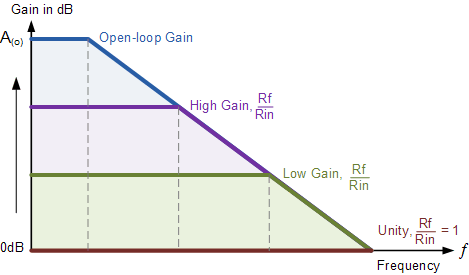
\includegraphics[scale = .5]{GBPpic.png}
    \label{GBPpic}
    \caption{\small The relationship between cutoff frequency (vertical dashed lines) and gain (horizontal lines), for a given op-amp. Lowering the gain of a circuit allows for a greater frequency range. Image courtesy of \textit{electronics-tutorials.ws}}
\end{figure}


% -------------------------- Methods and Materials ------------------------------
\section{Materials and Methods}
By using a National Instruments VirtualBench VB-8012 to take measurements and control input signals, and setting up a negative feedback loop as shown in Figure \ref{NFL}, the LM741 op-amp was characterized using frequencies ranging from 100Hz to 1MHz and two different gains. The input resistors were selected based on nominal values of 2k$\Omega$ and 20k$\Omega$ for setups 1 and 2, respectively. The feedback resistor was selected based on a nominal value of 200k$\Omega$ and was kept throughout the entire experiment. All resistors were measured before being integrated into the circuit. Channel 1 and channel 2 were setup to measure input and output voltages, and all grounds were connected to a common ground. Both experimental setups were based on the schematic shown in Figure \ref{NFL} and followed identical procedures. 

Beginning with a frequency of 100Hz, the experimental gain was calculated by taking ratio between measured values of output and input voltages. According the semi-theoretical model, the ratio between output and input voltage should be equal to ratio between feedback and input resistors. This served as the initial benchmark for comparing the experimental and semi-theoretical models.





% --------------------------------- Results ----------------------------------------
\section{Results}
This is where you show your results and key values

% --------------------------------- MATLAB ----------------------------------------
\newpage
\appendix
\section{MATLAB Script}
\lstinputlisting[style=Matlab-editor]{lab6.m}

\end{document}